\section{系统设计}

\subsection{需求分析与模块选型}

\subsubsection{系统功能需求分析}

根据一般企事业单位对于考勤事务的管理规范,本指纹考勤系统需要实现以下几种功能,通过上位机对于下位机中指纹识别模块保存的指纹信息进行注册与删除,下位机基于前者提供的指纹数据实现基于光学识别的指纹打开签到功能。

\subsubsection{系统方案设计与选型}

根据上述系统功能需求,以树莓派4B所提供的 bcm2711 作为中央处理芯片,指纹考勤系统主要由电源供电模块,声音反馈模块,USB转TTL串口通信模块,网卡模块。
系统总体设计方案如图2.1所示。

% https://www.processon.com/v/65ec0156778cc21034664557
\begin{figure}[ht]
    \centering
    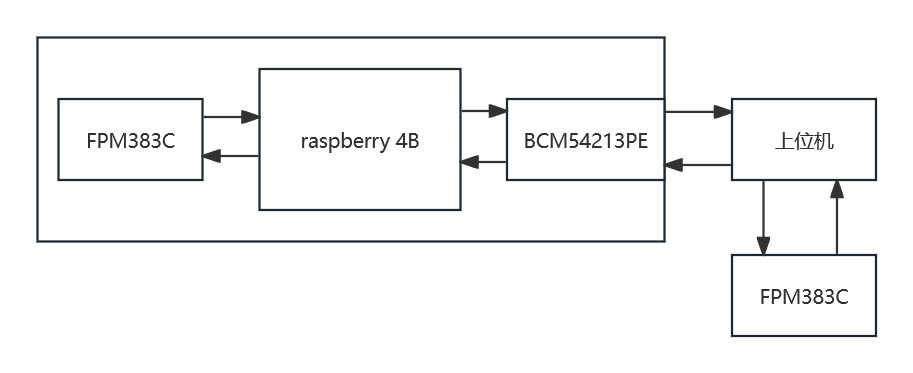
\includegraphics[width=\textwidth]{imgs/总体设计图.png}
    \caption{总体设计图}    \label{overall_design}
\end{figure}

\subsubsection{中央处理芯片选型}

树莓派4B使用的 bcm2711 是一种四核心64位ARM Cortex-A72架构CPU,主频高,能满足多种复杂计算需求以及满足大型程序运行需求。
树莓派4B还存在丰富而完善的接口,两个USb3.0接口,两个USB2.0接口,一个千兆网卡接口,一个HDMI接口,一个CSI接口和一个DSI接口,能够满足对于各种外设的连接需求。
树莓派4B还是树莓派第一个支持不通过 usb 直接访问网卡芯片实现网卡介入的开发板,这无形之中对于实现板载网卡驱动提供了很多帮助。

\subsubsection{指纹识别模块选型}

FPM383F识别指纹模块功耗低半导体面阵传感器是一款低功耗的光学指纹识别模块,支持对于60组光学指纹进行存储,其通过串口与中央处理器进行通信,在串口驱动方面,使用我开发的 arm\_gpio 库应当开发难度不难。

\subsubsection{通信模块选型}

    基于一般企事业单位对于考勤签到需求的需求,我计划提供多种不同的通信模块实现方便选用单位进行选择,
    其中传统基于 CH304 串口转 TTL 通信模块实现的简单串口通信主要适用于仅对于一两台设备进行支持的情况,
    而基于网卡模块间接通过网络方式拓展下位机数量的方式是主要计划实现的支持。
    针对于不同的预算管理需求,计划采用两种不同的方式实现网卡驱动,
    一种是基于 raspberry4B 板载 bcm54213PE 网卡芯片的驱动,
    另一种是基于 ENC28J60,一种基于 SPI 连接的外置 10BASE-T 以太网连接模块实现的。
    但是目前只实现了基于 BCM54213PE 网卡芯片驱动的支持。

\subsection{硬件设计}

    由于本实现相对来说比较轻量化,不太需要外部模块的支持,因此只是在面包板上完成了对应的实现,并没有画对应的板子。

    \begin{itemize}
        \item 信号回返模块:
            本模块主要实现的功能在基于树莓派电信号输出,实现简单的蜂鸣功能以提醒用户当前进行的打卡已经被正确识别。
            目前有两种实现的方法,一种是基于三极管实现的长延时信号灯,另外一种是基于无源蜂鸣器实现的。
        \item 指纹采集模块:
            本模块使用了现成的串口通信指纹识别模块予以完成。
        \item 网络通信模块:
            本模块主要使用了现有的树莓派板载 PHY 芯片 BCM54213PE 实现了对应的功能,同时
            还提供了串口替代的 USB 通信方法。
    \end{itemize}

\subsection{软件设计}

    由于本研究所采用的基础嵌入式应用程序所面对的的嵌入式应用场景相对较为单一,同时也是单应用程序单地址空间的。
    \footnote{虽然底层操作系统支持使用页表进行隔离,但是在应用层面上并没有使用到虚拟页表,只是在boot的时候使用了内核页表}
    因此整体软件设计相对较为简单,主要实现难度在驱动设计层面体现,具体内容与开发过程在第三章中进行呈现。
    在嵌入式应用层面只通过循环读取 UART 串口设备驱动反馈的数据,将其分析之后的结果通过由 ArceOS 包装底层以太网驱动实现的
    UDP 包经由 RJ-45 向上位机中运行的简单管理应用程序中发送。

    在上位机中通过简易的 python 客户端程序,对于嵌入式设备中传输的 UDP 包进行分析,实现基于 Sqlite 数据库的简单指纹信息 CRUD,打卡数据 CRUD,
    与一个基于命令行实现的打卡记录查询与导出应用程序。

    \begin{description}
        \item[指纹注册] 由上位机中自动完成指纹注册,通过上传命令,获取对应ID的指纹特征信息并以UDP包的形式下发到下位机中的指纹模块。
        
        指纹注册功能主要在上位机中完成,这主要是考量到在 HR 处实现人事登记等操作
        更加合乎一般企业的考勤流程。
        
        通过 0x0118 命令\ref{uart::auto-register},实现自动注册功能,该命令会自动完成采图、提取、拼接、保存等操作,
        在这个部分,通过对于回返包中 ID 以及注册进度的指示,在注册进度达到 0x64 时终止注册流程。

        \begin{table}[htbp]
            \resizebox{\textwidth}{!}{%
                \begin{tabular}{|l|l|l|l|l|l|l|l|}
                \hline
                \multicolumn{1}{|c|}{校验密码} & CMD类型 & CMD号 & 等待手指 & 按压次数 & ID\_H & ID\_L & 校验和  \\ \hline
                0x00 0x00 0x00 0x00        & 0x01  & 0x18 & 0x01 & 0x06 & 0xFF  & 0xFF  & 0xE2 \\ \hline
                \end{tabular}
            }
            \caption{自动注册命令用户层帧} \label{uart::auto-register}
        \end{table}

        在注册完成之后,通过上载命令\ref{uart::upload-info},向指纹模块获取特定 ID 号的指纹特征信息长度,
        然后再通过 \ref{uart::upload-data} 命令,从指纹模块获取对应分片的指纹特征信息。
        在将信息存储到数据库的同时,还通过 UDP 包的形式,将对应的数据发送到树莓派,树莓派再将对应指纹特征信息
        下载到树莓派对应的指纹模块上,由此完成了一次标准的指纹注册功能。

        \begin{table}[htbp]
            \resizebox{\textwidth}{!}{%
                \begin{tabular}{|l|l|l|l|l|l|}
                \hline
                \multicolumn{1}{|c|}{校验密码} & CMD类型 & CMD号 & ID\_H & ID\_L & 校验和  \\ \hline
                0x00 0x00 0x00 0x00        & 0x01  & 0x53 & 0x00  & 0x01  & 0xAB \\ \hline
                \end{tabular}
            } \caption{获取上传信息命令用户层帧} \label{uart::upload-info}
        \end{table}

        \begin{table}[htbp]
            \resizebox{\textwidth}{!}{%
            \begin{tabular}{|l|l|l|l|l|l|l|l|}
                \hline
                \multicolumn{1}{|c|}{校验密码} & CMD类型 & CMD号 & ID\_H & ID\_L & NUM\_H & NUM\_L & 校验和  \\ \hline
                0x00 0x00 0x00 0x00        & 0x01  & 0x51 & 0xFF  & 0xFF  & 0x00   & 0x00   & 0xAC \\ \hline
                \end{tabular}
            } \caption{获取指纹特征命令用户层帧} \label{uart::upload-data}
        \end{table}

        \item[指纹删除] Detailed explanation of functionality 2.
        \item[指纹考勤登记] Detailed explanation of functionality 3.
        \item[考勤记录读取] Detailed explanation of functionality 3.
    \end{description}
      

